\documentclass[a4paper]{scrreprt}
    
%% Language and font encodings and page settings
\usepackage[english]{babel}
\usepackage[utf8x]{inputenc}
\usepackage[T1]{fontenc}
\usepackage[a4paper,top=2cm,bottom=2cm,left=3cm,right=3cm,marginparwidth=2cm]{geometry}
\usepackage{float}

%% Packages
\usepackage{amsmath}
\usepackage{graphicx}
\usepackage[colorinlistoftodos]{todonotes}
\usepackage[colorlinks=true, allcolors=blue]{hyperref}
\graphicspath{{./img/}}

%% Title page settings
\title{Brexit Vs Good Friday}
\subtitle{"Defend the Good Friday Agreement"}
\author{Cian Gannon}
\titlehead{\centering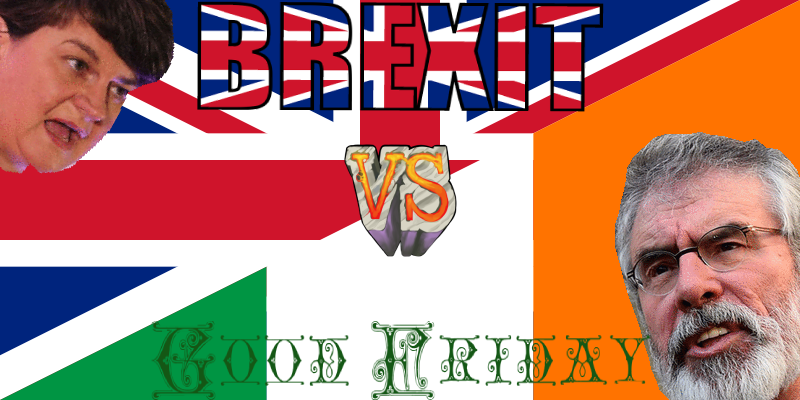
\includegraphics[width=10cm]{header}}

%% Page settings
\pagestyle{headings}

%% Start of document
\begin{document}

%% Render title settings
\maketitle

%% Start abstract page
\begin{abstract}

%% Center everything on this page
\centering

%% Image of Gerry Adams

\includegraphics[width=2.7cm]{gerrylad}

%% Quick run down of the game concept
Brexit Vs. Good Friday is a satirical representation of the current Brexit debacle and Ireland's core involvement in it due to the Good Friday Agreement. 
Brexit Vs. Good Friday is a top-down shooter that will expand the genre and also involve the most loved elements of other shooters.

%% Note in bottom left of abstract page
\begin{flushleft}
\noindent
\null\vfill
Game Design Document: \\
Brexit Vs Good Friday \\
Created by - Cian Gannon \\
Student ID - G00337022 \\
\today
\end{flushleft}

\end{abstract}

%% Render table of contents
\tableofcontents

%% Chapter 1
\chapter{Overview}

\section{Main Concept}
Brexit Vs. Good Friday is a satirical representation of Brexit and the hysteria surrounding it. 
It's a top-down shooter where the user plays Gerry Adams a politician who returns from retirement in order to save what many hold dear.

\section{Core Selling Points}

\subsection{Survival Elements}
\begin{description}
\item[$\bullet$] The player must dodge incoming fire.
\item[$\bullet$] The aim of the game is to protect Good Friday in a countdown until the UK leaves the EU and therefore single market. 
If the player fails in their attempt by getting hit then Good Friday will be removed and the player fails. 
If the player survives the countdown then the Good Friday is upheld.
\end{description}

\subsection{Humor}
\begin{description}
\item[$\bullet$] The game is made to be humorous. Its take on Brexit that is a core issue currently in the EU is used to make all players on both sides laugh.
\item[$\bullet$] The game is created to be topical, games that are topical tend to be a hit with players.
\end{description}

\subsection{Top Down Shooter}
\begin{description}
\item[$\bullet$] Top-down shooter which needs basic input so the game will be comfortable to play on mobile or desktop.
\item[$\bullet$] Top-down games have been around for generations of consoles and have evolved over time. Brexit Vs. Good Friday aims to take the general style and improve upon it.
\end{description}

%% Chapter 2
\chapter{References} 

\section{Games Examined}

I analysed three games as part of my investigation as to what makes a shooter fun and what is unique about a top-down one.

\subsection{GTA}

\begin{figure}[H]
\centering
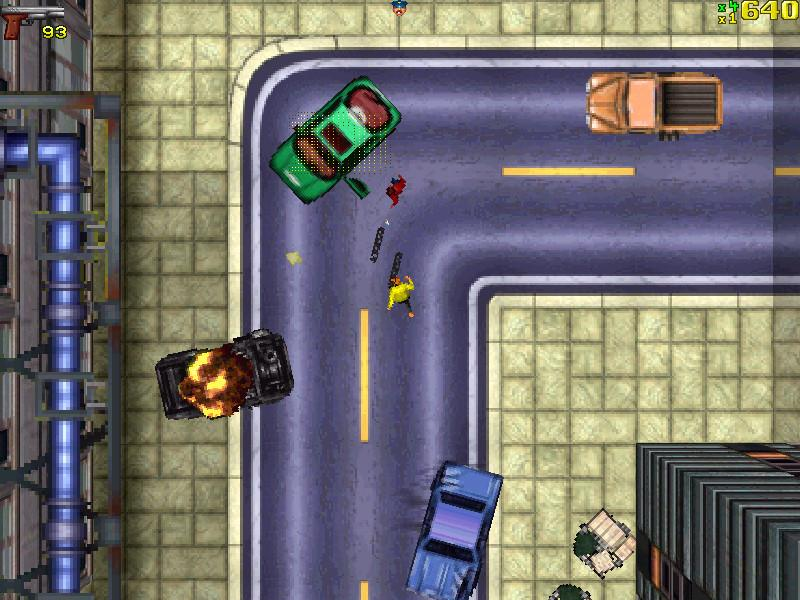
\includegraphics[width=0.70\textwidth]{gta1.jpg}
\caption{\label{fig:art} GTA 1}
\end{figure}

\subsubsection{Core Features}
\begin{description}
\item[$\bullet$] Single Player
\item[$\bullet$] Top-down Shooter
\item[$\bullet$] Open world
\item[$\bullet$] Action/Adventure
\item[$\bullet$] 2D
\end{description}

\subsubsection{Note}
Grand Theft Auto is a top-down action shooter developed by Rockstar Games. Set in an open world approximation of Ney York city.
A basic top-down game that revolutionized the genre by adding an open world.
What truly made Grand Theft Auto stand out from other game of the period are it's ease of use controls. 
The pick up and play controls allowed users of all experience levels get to grips with the game. \\\\
I will be adapting GTA's ease of control and fluid movement as part of my development.

\subsection{Doom}

\begin{figure}[H]
\centering
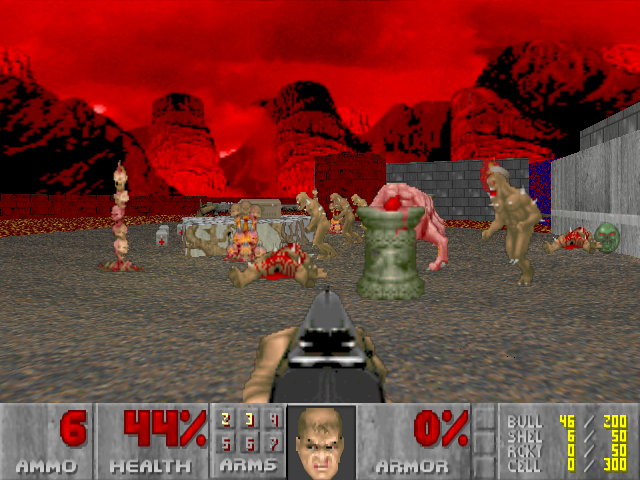
\includegraphics[width=0.70\textwidth]{doom.png}
\caption{\label{fig:art} Doom}
\end{figure}

\subsubsection{Core Features}
\begin{description}
\item[$\bullet$] Single Player
\item[$\bullet$] First Person Shooter
\item[$\bullet$] Linear/Semi Open World
\item[$\bullet$] Action
\item[$\bullet$] 'Fake' 3D/ 2.5D
\end{description}

\subsubsection{Note}
Doom is a first-person shooter developed in 1993. 
Although my game is going to be top down, taking inspiration from the first person shooter genre and adapting them for Brexit Vs. Good Friday.
Doom consists of a constant stream of enemies in a fast-paced environment that always keeps the player busy.
Doom has no story and keeps the player entertained with gameplay alone. \\\\
I will be adapting Doom's enemy variety and enemy frequency.

\subsection{Hotline Miami}

\begin{figure}[H]
\centering
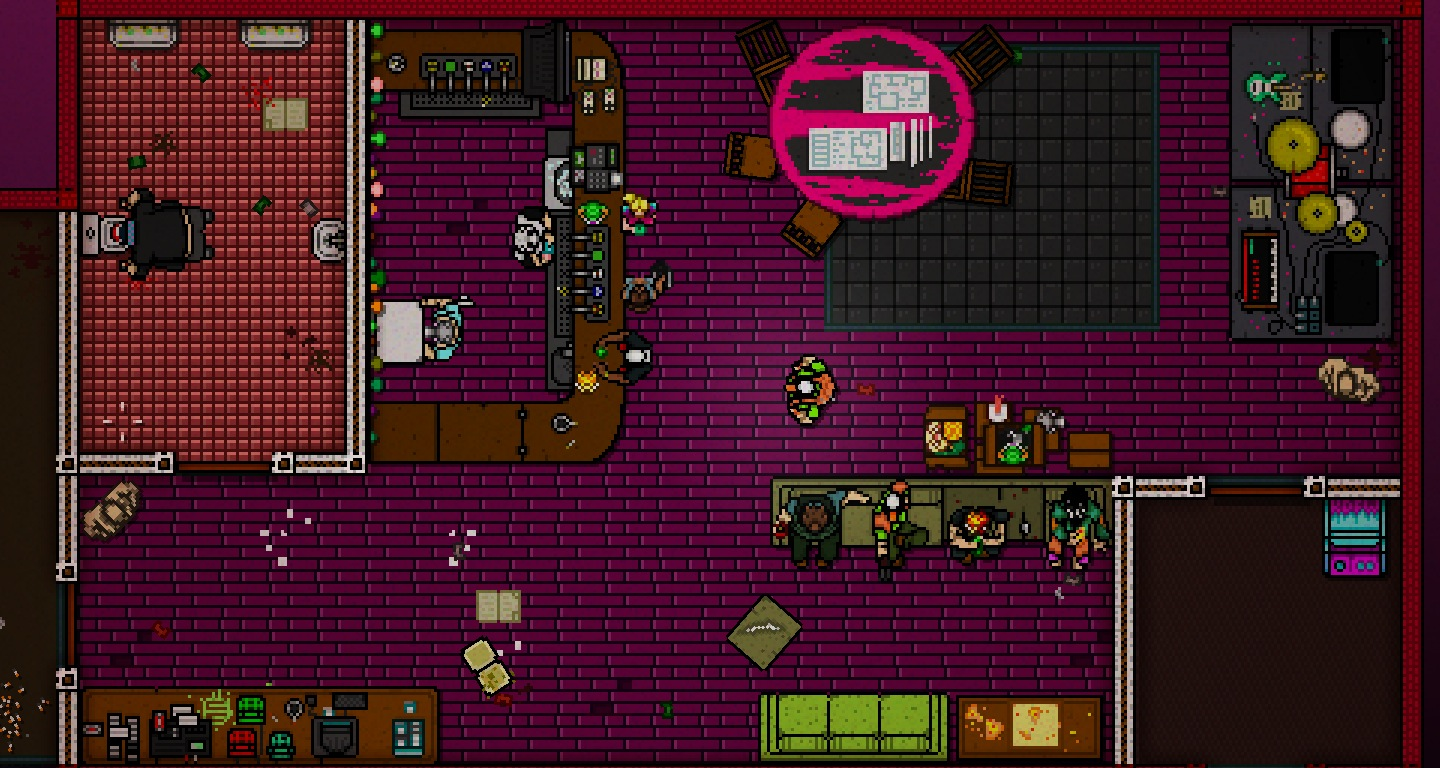
\includegraphics[width=0.70\textwidth]{hotline-miami.jpg}
\caption{\label{fig:art} Hotline Miami}
\end{figure}

\subsubsection{Core Features}
\begin{description}
\item[$\bullet$] Single Player
\item[$\bullet$] Top-Down Shooter
\item[$\bullet$] Semi Open World
\item[$\bullet$] Action
\item[$\bullet$] 2D
\end{description}

\subsubsection{Note}
Hotline Miami is a top-down action shooter that throws more and more enemies at the player in order to increase the difficulty for the player. 
The player has a choice of weaponry to deal with the onslaught of ever increasing enemies.    

%% Chapter 3
\chapter{Specification}

\section{Target Group}

\begin{description}
\item[$\bullet$] The target group is a younger generation 35 and under.
\item[$\bullet$] Target platform is mobile devices specifically windows phones.
\item[$\bullet$] Interested in the current Brexit negotiations and just want to get away from the seriousness of it all.
\item[$\bullet$] People who understand Irish politics and the humor around it.
\end{description}

\section{Genre}
Brexit Vs. Good Friday is a top-down satirical shooter based on the current Brexit debate.

\section{Art Style}

\begin{center}

\includegraphics[width=4.5cm]{celtic-knot}

\includegraphics[width=5cm]{celtic-knot-arrow}

\includegraphics[width=4.5cm]{celtic-knot}
\begin{figure}[H]
\centering

\includegraphics[width=4.5cm]{start-game}
\caption{\label{fig:art} Game Menu Concept Art}
\end{figure}
\end{center}

I'll be going for a traditional Celtic art style as this game will portray the Irish viewpoint of Brexit. 
It will mix Celtic symbols for user interface 'fluff' and use Gaelic font type for menus.

\begin{figure}[H]
\begin{addmargin}[13.5em]{0em}
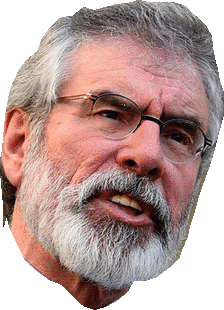
\includegraphics[width=1.5cm]{gerry-right}
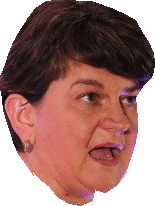
\includegraphics[width=1.5cm]{arlene}

\includegraphics[width=1.5cm]{tess}
\end{addmargin}
\caption{\label{fig:art} Character Concept Art}
\end{figure}

\begin{flushleft}
The game will use satirical representations of politicians throughout the game as player characters and non-player characters (NPCs).
\end{flushleft}

\begin{flushleft}
The game will heavily lean on Irish humor surrounding our history and politics.
\end{flushleft}

%% Chapter 4
\chapter{Gameplay and Setting}

\begin{center}
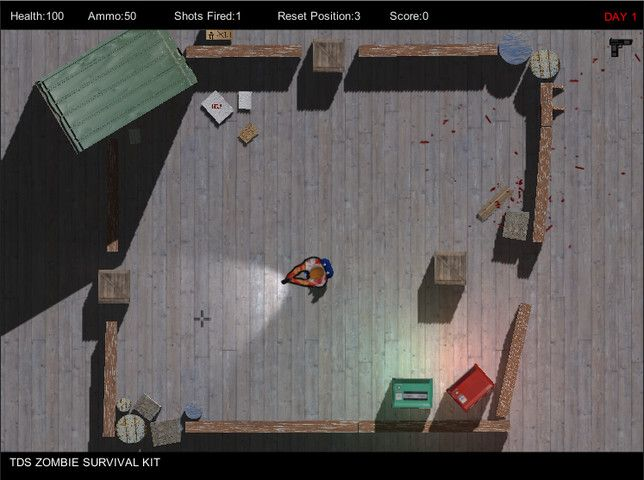
\includegraphics[width=7cm]{top-down}
\end{center}

The game is centered around the player who moved around the screen and defends against incoming enemies.
The player will have special abilities that they may use in addition to their main offensive weapon.

\section{Mood and Emotions}

The mood of the game is to be humorous.
The characters are over the top representations of real politicians the main menu will feature Irish in-jokes.
The who premise of the game is to make the user laugh while also delivering compelling gameplay.

\section{Characters in the Game}

\begin{figure}[H]
\begin{addmargin}[13.5em]{0em}
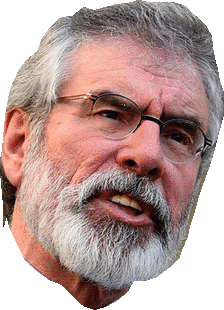
\includegraphics[width=1.5cm]{gerry-right}
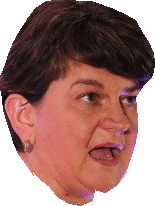
\includegraphics[width=1.5cm]{arlene}

\includegraphics[width=1.5cm]{tess}
\end{addmargin}
\caption{\label{fig:art} Character Concept Art}
\end{figure}

The game will feature real-world politicians in an over the top satirical outlook.
The game will feature Gerry Adams as the main protagonist/antagonist (Depending on the user's outlook)
The game will use politicians from the UK as enemies that are trying to undermine the Good Friday Agreement.

\section{Main Objective}

Survive an onslaught of enemies while a counter is on screen. 
The player will have to dodge oncoming fire while also fireing back at the oncoming enemies.

\section{Core Mechanics}

\begin{description}
\item[$\bullet$] Tactical Maneuvering \\
The player will have to dodge incoming fire from enemies. While also trying to line up shots on enemies.
\item[$\bullet$] Resource Management \\
The player will have to manage their ammo and other abilities. The player will also have to manage their time as the clocks counts down.
\item[$\bullet$] Survival \\
The player must survive hordes of enemies that will fire at them and try and eliminate the player. The player must sruvive while a clocks runs down.
\end{description}

\section{Controls}

\subsection{Mobile}

\begin{center}

\includegraphics[width=7cm]{mobile}
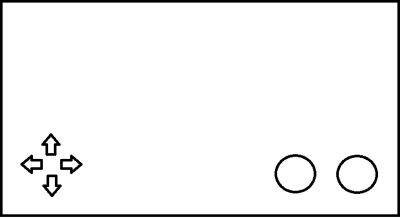
\includegraphics[width=7cm]{mobile-controls}
\end{center}

The player will be controlled by using touchscreen on a mobile device. \\\\
Directional pad is used to control player movement.\\
Left and right buttons used to fire and use secondary ability.

\subsection{PC}

\begin{center}
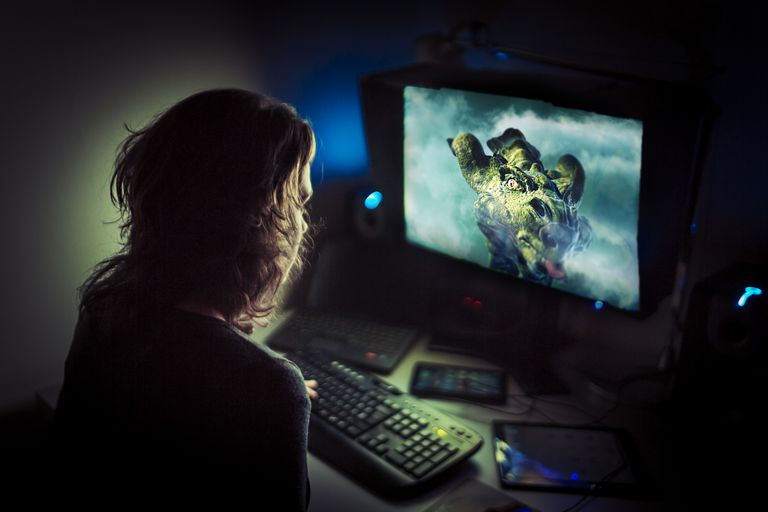
\includegraphics[width=7cm]{pc-gaming}
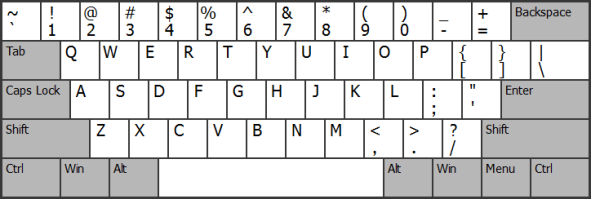
\includegraphics[width=7cm]{pc-controls}
\end{center}

The game will be developed on PC so controls will be tested with keyboard and mouse and as such will work in the final release. \\\\
W,A,S,D will be used as directional buttons as they are the standard movement keys in PC gaming. \\
Space will be primary ability, which is to shoot at enemies. \\
E will be used to execute the players second abilities.

\subsection{Xbox One}

\begin{center}
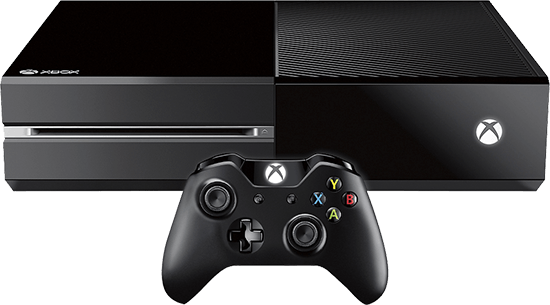
\includegraphics[width=7cm]{Xbox-one}
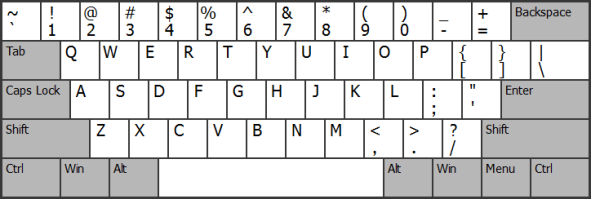
\includegraphics[width=7cm]{pc-controls}
\end{center}

The game will be compatible with Xbox One by using a keyboard and mouse that are connected to the console. \\\\
Just as above with the PC version, the Xbox One version will use a keyboard layout. \\
W,A,S,D will be used as directional buttons as they are the standard movement keys in PC gaming. \\
Space will be primary ability, which is to shoot at enemies. \\
E will be used to execute the players second abilities.

%% Section 5
\chapter{Front End}

\section{Start Screen}

The start screen will feature traditional Irish/Celtic symbols and font.\\
The start screen will feature background images of Ireland and its politicians while ambient music plays waiting for the player to interact with the game.\\
Once the player interacts with the game they will transition to the main menu.

\section{Menus}

There will be two menu types in the game for the user to interact with.\\
The main menu and the pause menu.

\subsection{Main Menu}

\begin{center}

\includegraphics[width=4.5cm]{celtic-knot}

\includegraphics[width=5cm]{celtic-knot-arrow}

\includegraphics[width=4.5cm]{celtic-knot}
\begin{figure}[H]
\centering

\includegraphics[width=4.5cm]{start-game}
\caption{\label{fig:art} Game Menu Concept Art}
\end{figure}
\end{center}

The main menu is where the user will have multiple options.

\begin{description}
\item[$\bullet$] Start Game \\
Start Game option will start a new game from the start.
\item[$\bullet$] Chapter Select \\
Chapter Select option allows the user to select a chapter.
\item[$\bullet$] Options \\
Options allow the user to change game options such as audio volume.
\item[$\bullet$] Quit \\
Quit exits the game and closes it.
\end{description}

\subsection{Pause Menu}

\begin{figure}[H]
\centering
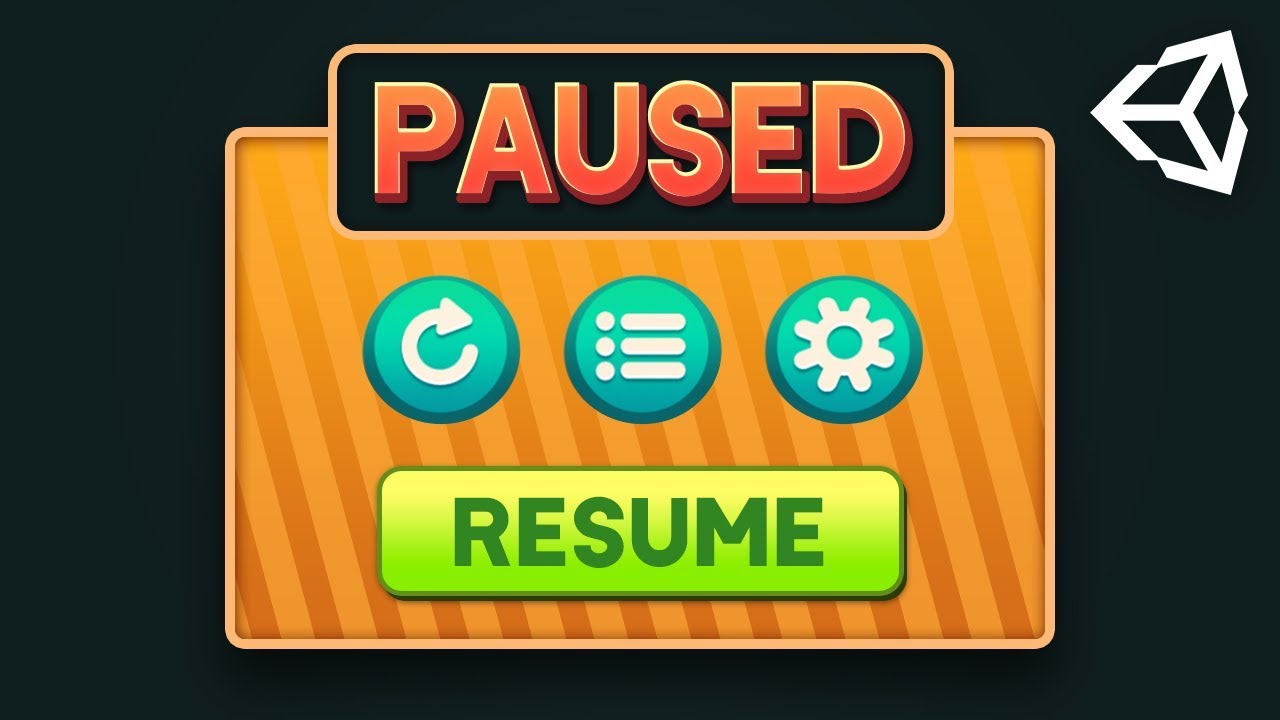
\includegraphics[width=0.70\textwidth]{pause}
\caption{\label{fig:art} Pause Menu}
\end{figure}

The pause menu will be available when the user pauses the game while they are playing. When paused the user will have an option to quit or resume.
Quitting will bring the user back to the menu and resuming will bring the user back to the game when they left off.

\section{End Screen}

The end screen will transition the user from one level to another using a 'cut-scene'. If the user finished the game they will be greeted by you won message.
Music will play to congratulate the player on their completion of the journey.


%% Chapter 6
\chapter{Technology}

\includegraphics[width=0.50\textwidth]{Unity}

The game will be developed in unity for UWP (Universal Windows Platform).

\section{Target Systems}

\begin{center}
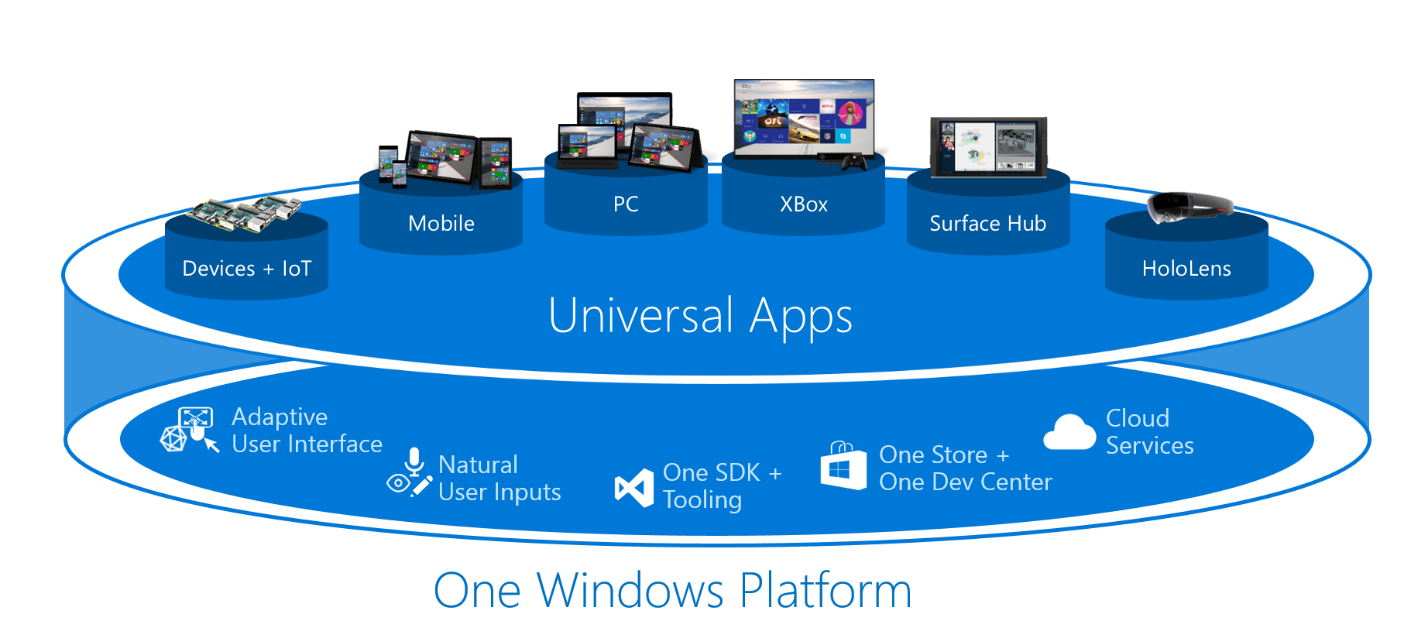
\includegraphics[width=12cm]{uwp}
\end{center}

UWP (Universal Windows Platform) devices will be the target devices. The game will use UWP (Universal Windows Platform) as it will be compatible with windows phones, Xbox and PC.

\section{Development Systems/Tools}

A computer will be used as the development system.\\
Unity will be the game engine that will be used to develop the game.\\

\subsection{Art Development}

\begin{description}
    \item[$\bullet$] For developing the logo and all character sprites I will use \href{https://www.photopea.com/}{Photopea}.
    \item[$\bullet$] I will source images from \href{https://images.google.com/}{Google Image Search}.
\end{description}

\subsection{Programming/Development}

\begin{description}
    \item[$\bullet$] \href{https://unity3d.com/}{Unity} will be the game developement environment I will use to develop the game.
    \item[$\bullet$] \href{https://visualstudio.microsoft.com/}{Visual Studio} is the IDE (Integrated development environment) used to edit C\# files used by the game.
\end{description}

\subsection{Source Control}

\begin{description}
    \item[$\bullet$] I will use \href{https://git-scm.com/}{git} as my source control.
    \item[$\bullet$] I will use \href{https://github.com}{Github} to store my source code using \href{https://git-scm.com/}{git}.
    \item[$\bullet$] I will use Git Bash which is included with a \href{https://git-scm.com/downloads}{git}.
\end{description}

\subsection{Documentation}

\begin{description}
    \item[$\bullet$] A game design document (this document) available on the \href{https://github.com/cian2009/UnityGame}{project Github}. The game design document will use \href{https://www.latex-project.org/}{Latex} as the editor and then I will render it in a pdf format.
    \item[$\bullet$] A read me will be available on github detailing what was used in development, how to open the source code in unity and other important information for other developers to pick up.
\end{description}

\end{document} 